%&LaTeX
%\documentclass[border=5pt]{standalone}
\documentclass[12pt]{report}
\textheight  9.5 in
\topmargin  -1.2 in
\textwidth 7.1 in
\oddsidemargin -.3in



\usepackage{amsmath}
\usepackage{amsthm}
\usepackage{amssymb}
\usepackage{fancybox}
\usepackage{bm}
\usepackage{hyperref}
\usepackage{graphicx}
\usepackage{booktabs}
\usepackage{multirow}
\usepackage{subcaption}

\graphicspath{{figure/}}

\begin{document}
\begin{center}
\line(1,0){500}\\
\Large{\textbf{Glassdoor Data Science Internship Project}}\\[2pt]
\large{by \textbf{Jin Xie} (bruce.jinxie@gmail.com)}\\[4pt]
\small{April 9, 2018}
\line(1,0){500}
\end{center}

\noindent All of the code, prediction and report files can be found in the zip file attached to the email or the github page below:
\begin{itemize}
	\item \url{https://github.com/kof900/Glassdoor-Intern-Project}
	\begin{itemize}
		\item ``\verb|input|" folder contains the Train and Run data.
		\item ``\verb|output|" folder contains the Run data with prediction of likelihood of ``isWon".
		\item Jupyter notebook file, ``\verb|Glassdoor Data Challenge.ipynb|", is in the default path.
		\item ``\verb|report|" folder contains the report latex and pdf file.
	\end{itemize}
\end{itemize}

\noindent Answers to Question 3 are in the following.
\begin{enumerate}
	\item[\textbf{a.}] First  evaluate  the  data  -­  what  initial  observations  can  you  make  from  this  data?  Are  there  any  concerns  about  the  data?
	
	This is a binary classification problem. In general, a logistic regression model should work. The predictors have both categorical and continuous variables. There are a lot of missing values in the dataset. I also note that it's an imbalanced binary classification problem. ``isWon=True" only takes 10.9\% of all the observations in the Train data. I have several concerns regarding the data.
	
	\begin{enumerate}
		\item Imbalanced Binary Classification Problem.
		
		Data is very unbalanced. Only 10.9\% of the observations are the winning cases (``isWon=True") in the train data. The remaining 89.1\% are all failure cases (``isWon=False").
		
		\begin{table}[h!]
			\centering
			\caption{Case Proportion in the Train Data}
			\resizebox{1.1\textwidth}{!}{\begin{minipage}{\textwidth}
					\centering
					\begin{tabular}{lc}
						\toprule[1.5pt]
						Case &  Proportion \\ \midrule
						isWon &  0.109 \\
						nonWon &  0.891 \\ \bottomrule[1.5pt]
					\end{tabular}
			\end{minipage}}
		\end{table}
		
		It suggests us that accuracy can be deceptive. If we predict every case is failure case, i.e. ``isWon=False", we could have a 89.1\% accuracy. But it's meaningless. We should use some criteria such as AUC or FNR.
		
		\item Duplicates in the Train Data.
		
		``EmployerId" should be unique. However, I observe that there are 2 observations in the train data having the same "employerId". The ``employerId" is ``2bX4R".
		
		\item Some ``employerId" in the Run Data can be found in the Train Data.
		
		In other words, we could potentially cheat on ``employerId". We just use the value in the Train data as the prediction in the Run data since they can be found in the Train data. I did not do this since it is not the purpose of this project. But one could dramatically increase the model performance by cheating in this way.
		
		\item Missing Values.
		
		There are so many missing values in the Train Data. Some methods such as tree methods will be able to deal with missing values directly. However, some algorithm such as logistic regression model cannot deal with missing values unless imputing the missing values beforehand. Otherwise we will have to delete all the cases containing any missing values. The missing values can be a big problem
		
		\begin{table}[h!]
			\centering
			\caption{Missing Values in the Train Data}
			\resizebox{1.0\textwidth}{!}{\begin{minipage}{\textwidth}
					\centering
					\begin{tabular}{lcc}
						\toprule[1.5pt]
						       Feature         & Missing Count & Proportion \\ \midrule
						        isWon          &       0       &   0.000    \\
						      subsidiary       &       0       &   0.000    \\
						       numJobs         &       0       &   0.000    \\
						    basePayAmount      &       0       &   0.000    \\
						   has\_interviews     &       0       &   0.000    \\
						      timeOnSite       &       0       &   0.000    \\
						      employerId       &       0       &   0.000    \\
						       ATS\_\_c        &       4       &   0.000    \\
						  employeesTotalNum    &      172      &   0.010    \\
						       Industry        &      602      &   0.036    \\
						  RespondedContacts    &     2674      &   0.158    \\
						    intDifficulty      &     2839      &   0.168    \\
						     intDuration       &     3149      &   0.186    \\
						     freshContent      &     3292      &   0.195    \\
						      followers        &     3292      &   0.195    \\
						     contentCount      &     3292      &   0.195    \\
						        awards         &     3292      &   0.195    \\
						        photos         &     3292      &   0.195    \\
						      starRating       &     3956      &   0.234    \\
						monthOfSignupPageViews &     4708      &   0.279    \\
						        clicks         &     6037      &   0.357    \\ \bottomrule[1.5pt]
					\end{tabular}
			\end{minipage}}
		\end{table}
	
	\item Outliers.
	
	There a lot of outliers in the Train data. And it could harm the analysis.
	
	\item Predictor is skewed and in large scale.
	
	Some predictors such as clicks have a very large range and the scale is very large. They are also very skewed. It suggests that some transformation may be needed. I did $\log(x)$ or $\log(x+1)$ transformations on some predictors depending on whether it's skewed and has zero values. For example, for ``employeesTotalNum", the original and $\log$ transformed data histograms can be found as below.
	\begin{figure}[h!]
		\begin{subfigure}[h]{0.41\linewidth}
			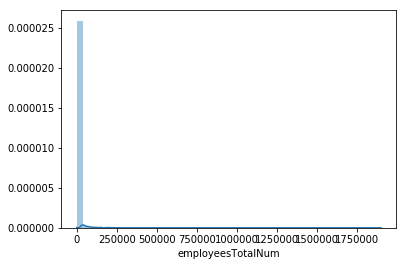
\includegraphics[width=\linewidth]{skew.png}
			\caption{Original}
		\end{subfigure}
		\hfill
		\begin{subfigure}[h]{0.4\linewidth}
			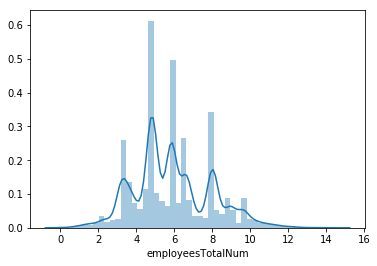
\includegraphics[width=\linewidth]{transform.png}
			\caption{$\log$ Transformed}
		\end{subfigure}%
	\end{figure}
		
	\end{enumerate}

	
	\item[\textbf{b.}] Imagine  you  are  presenting  your  results  to  a  non-­technical  audience.  Summarize  your 
	findings  -­  What  are  the  top  3  insights  that  you  can  draw  from  this  data  set?  Share  your 
	plots  and  findings.
	
	\begin{enumerate}
		\item The higher ``monthOfSignupPageViews" the employer has, the higher likelihood it would have to become a client.
		
		\begin{figure}[h!]
			\caption{winning likelihood vs. Log monthOfSignupPageViews}
			\centering
			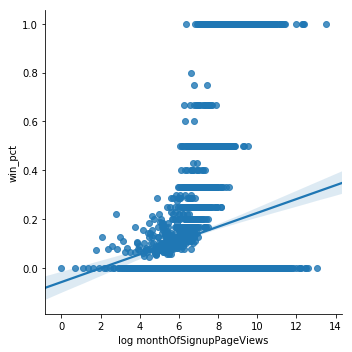
\includegraphics[scale=.8]{top1.png}
			\label{top1}
		\end{figure}
	
	From the above plot, we can easily see that with ``$\log$ monthOfSignupPageViews" increasing, the winning likelihood also has an increasing trend.
	
	\item The higher ``clicks" the employer has, the higher likelihood it would have to become a client.
	
	\begin{figure}[h!]
		\caption{winning likelihood vs. Log clicks}
		\centering
		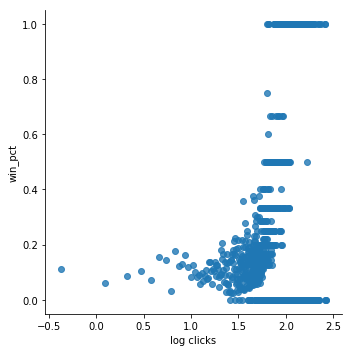
\includegraphics[scale=.7]{top2.png}
		\label{top2}
	\end{figure}
	
	From the above plot, we can easily see that with ``$\log$ clicks" increasing, the winning likelihood also has an increasing trend.
	
	\item I made a barplot using winning likelihood by industries as in Figure \ref{bar}.
	
	\begin{figure}[h!]
		\caption{winning likelihood by industries (red vertical line is the average for all)}
		\centering
		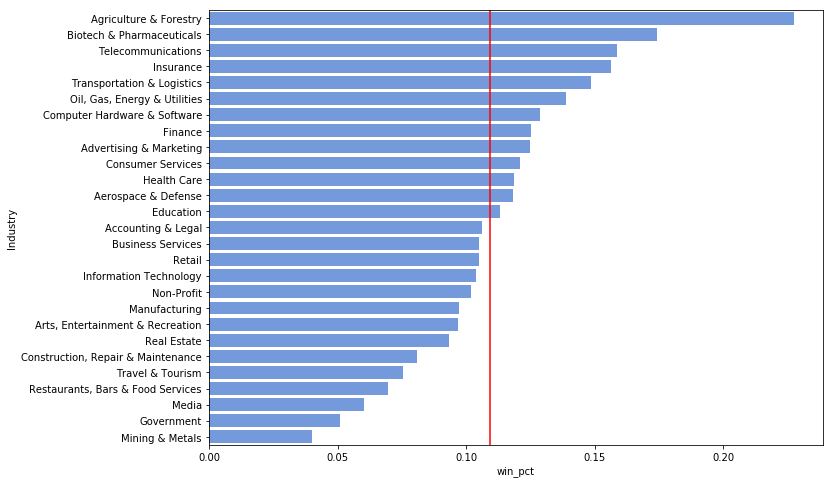
\includegraphics[scale=.6]{top3.png}
		\label{bar}
	\end{figure}
	
	Clearly, ``Agriculture \& Forestry" is the industry area that has the highest winning likelihood. We should put more effort on this industry area rather than ``Mining \& Metals" industry area, which has the lowest winning likelihood.
	
	\end{enumerate}

	\item[\textbf{c.}] Train  and  test  a  model  to  predict  how  likely  an  account  will  be  won  (meaning  they 
	become  a  paying  customer).  You’re  welcome  to  just  pick  a  few  features  (please  describe 
	your  reasoning  in  picking  the  features).  For  this  task,  use  the  data  set 
	\verb|data_challenge_traindata.csv|. 
	
	For this part, I trained 3 different models.
	\begin{enumerate}
		\item Gradient Boosting Tree method using the cutting-edge python library \href{https://github.com/Microsoft/LightGBM}{LightGBM}.
		
		\item Logistic Regression only with the features that don't have any missing values.
		
		\item Logistic Regression with imputing the missing values using mean value.
	\end{enumerate}
	
	Their performances will be discussed in the next questions.
	
	\item[\textbf{d.}] Briefly  describe  in  a  few  words:  How  well  does  the  model  work?  Which  are  the  most 
	important  features?  What  about  accuracy? 

	As we discussed in question \textbf{a}. Accuracy is deceptive since we can easily get 89.1\% accuracy by predicting every case as failure. Instead, we use Area Under the Curve (AUC) from Receiver Operating Characteristic (ROC) curve.
	
	\begin{figure}[h!]
		\caption{ROC curve for 3 methods}
		\centering
		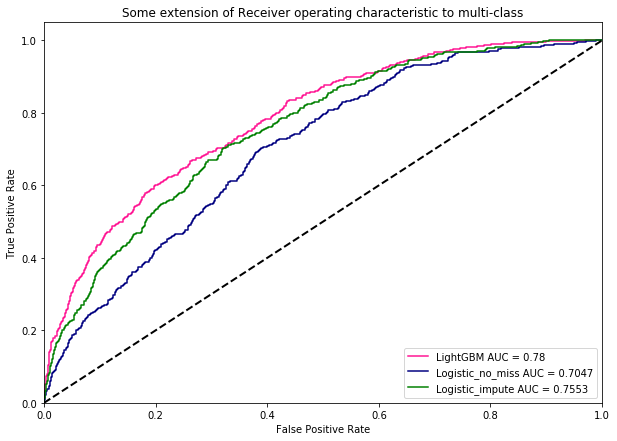
\includegraphics[scale=.6]{roc.png}
		\label{roc}
	\end{figure}

	As we can observe from the ROC curve (Figure \ref{roc}), LightGBM outperforms both Logistic Regression models. And Logistic Regression model with imputation has better performance than Logistic Regression only on non-missing features.
	
	\begin{figure}[h!]
		\caption{Feature importance from LightGBM}
		\centering
		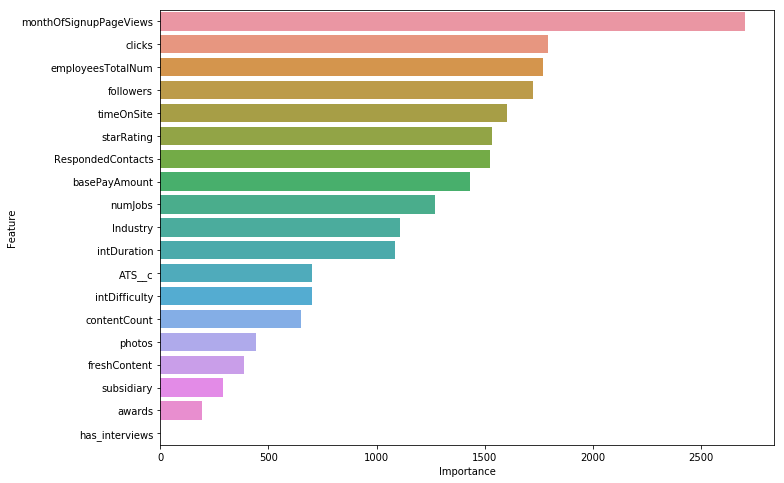
\includegraphics[scale=.6]{imp.png}
		\label{imp}
	\end{figure}

	Figure \ref{imp} is the feature importance plot from LightGBM model. We can see that ``monthOfSignupPageViews", ``clicks" and ``employeesTotalNum" are the top 3 important features.
	
	\newpage
	\item [\textbf{e.}] Run  your  model  on  the  dataset  \verb|data_challenge_rundata.csv|.  What  insights  can  you 
	draw?
	
	After fitting the model to the Run data (\verb|data_challenge_rundata.csv|), I list the top 10 ``employerId" that has the highest winning likelihood. I also list the bottom 10 ``employerId" that has the lowest winning likelihoods. In other words, we should reach out more actively to the top 10 employers.
	
	\begin{table}[h!]
		\centering
		\caption{Top and Bottom Prediction on Winning Likelihood in the Run Data}
		\resizebox{1.1\textwidth}{!}{\begin{minipage}{\textwidth}
				\centering
				\begin{tabular}{cccc}
					\toprule[1.5pt]
					\multicolumn{2}{c}{Top} & \multicolumn{2}{c}{Bottom} \\ \midrule
					employerId &  Winning Likelihood & employerId &  Winning Likelihood  \\ \midrule
					uPI8q &  0.896 & 8tMdC &  0.003 \\
					DSjqi &  0.882 & yW4fr &  0.004 \\
					4VJt2 &  0.875 & 4bAHQ &  0.004 \\
					Z7ZPH &  0.825 & VQP0r &  0.004 \\
					tRv6U &  0.802 & TUUsk &  0.004 \\
					Dgawj &  0.792 & MDehi &  0.004 \\
					4363z &  0.791 & Mc024 &  0.004 \\
					zpIcy &  0.791 & 6p9qR &  0.004 \\
					i3lry &  0.790 & yYrbE &  0.004 \\
					iQNj7 &  0.785 & cDiJK &  0.004 \\ \bottomrule[1.5pt]
				\end{tabular}
		\end{minipage}}
	\end{table}

	\item[\textbf{f.}] If  you  run  out  of  time/had  extra  time:  Please  explain  the  next  steps  you  would  take. 
	
	I have a few thoughts in my mind for future works.
	\begin{enumerate}
		\item Screen out outliers by looking at each feature.
		\item Use EM algorithm to impute the missing values rather than just using the mean.
		\item Try several other different models and do model ensemble.
	\end{enumerate}

\end{enumerate}

\end{document}
